%!TEX ROOT=main.tex

\section{Analysis of the System}
As was discussed in the Introduction \ref{chapter:introduction}, the main goal of this work is the soil moisture sensor hardware with the accompanying firmware and a proof-of-concept application.

With that being said, one can easily discern separate sub-tasks within this broader goal - mainly the fact, that the communication aspect can be separated from the sensor itself (see Figure \ref{fig:device-split}) a practice commonly seen in the industry.

\begin{figure}
    \includesvg[width=\textwidth]{fig/device-split.drawio.svg}
    \caption{\label{fig:device-split}Logical high level building blocks of most modern sensors}
\end{figure}

Separating these two concerns not only logically, but also on the hardware level, will bring many advantages - future sensor implementations can be made with only effort being put into the sensor itself; the wireless part and most of the testing and regulation overhead can be solved once, not repeated for every sensor type; once a sensor compatible with the interface exists, it can be made compatible with future versions of the interface - to list a few.

While this work is mainly concerned with the soil moisture sensing application, having a LoRa compatible unit, which is capable of OTA updates and has enough processing power to handle most sensing and simple control task, while being power-efficient enough to be battery powered, is an interesting sub-goal of this work.

The following sections will go through the process of finding requirements for such hardware and explain the compromises made.

\section{Generic LoRa module requirements}
\subsection{\label{section:ota-update-support}Over The Air update support}
There are two general approaches to implementing OTA updates \cite{bucklin_brown_over--air_2024,noauthor_android_2024}. First is to split the firmware into a so-called Bootloader, a binary which runs before the main application and implements a way to communicate with the master node, such that it is able to overwrite the application. The application usually also needs to communicate with the master node in order to transmit sensor data and accept commands, which leads to duplication of all the driver and protocol logic required to use the communication interface.

The first option provides some level of separation between the application and the Bootloader, which could be useful in cases where the application is in some ways ``untrusted'', either due to security measures limiting the potential impact of bugs, or because it is actually provided by a different vendor and so on. This could be especially valid for cases, where the processor provides privileged execution modes etc.

But it also cuts the other way, since this approach hinders the upgradeability of the device itself, because now this relatively large Bootloader with all the error prone interface handling is locked in and unable to be updated remotely, unless, of course, the application also implements a way to update the Bootloader, but this defeats any potential security benefits, unless a sophisticated authentication method is employed in both the Bootloader and the Application, which leads to even more duplication.

This brings us to the second option, which also consists of a Bootloader and the Application, but here the Bootloader is much simpler, it only implements the bare minimum that is required to take a newer version of the application and overwrite the currently active one, see Figure \ref{fig:bootloader-flash}. However, if the Bootloader is unable to communicate with the master node, this means that the Application needs to download the new binary and store it somewhere locally on the end-node.

This is usually a challenge for embedded devices, where the built-in FLASH memory, in which the application is stored and from which it is executed, is generally just about able to fit the Bootloader and the Application and rarely would be able to accommodate two copies of the binary.

Integrating additional memory increases the cost, but it can be used for other proposes besides OTA updates, such as storing configuration, calibration data and logs, or if the application integrates some sort of graphical display, may be required to store the assets, such as images and fonts.

Perhaps the most important benefit is that, with proper Bootloader the support \cite{drogue_iot_firmware_2024,embassy_project_documentation_bootloader_2024}, the application binaries can be swapped instead of the old one being deleted, which opens up the possibility of rolling back unsuccessful updates, that could be considered a crucial feature in some applications and is not practical to do in the first OTA approach that was presented.

\begin{figure}
    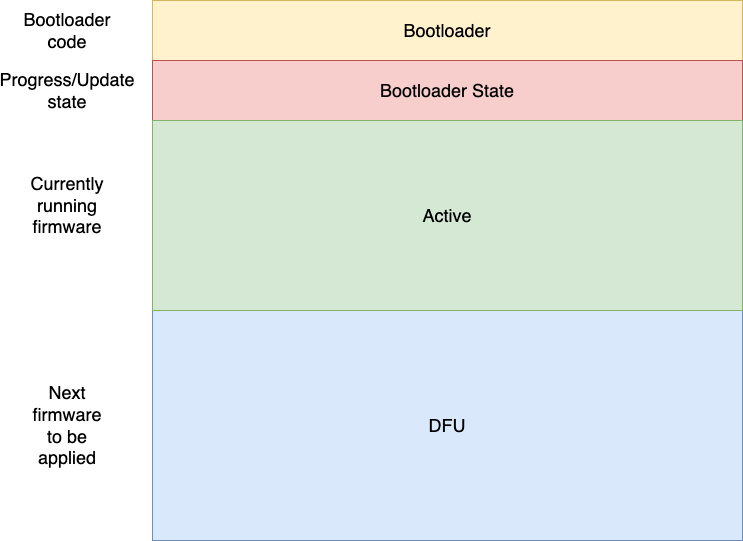
\includegraphics[width=.6\textwidth]{fig/bootloader_flash.png}
    \caption{\label{fig:bootloader-flash}The bootloader divides the storage into 4 main partitions}
\end{figure}

\subsection{\label{section:application-case-studies}Generic LoRa module applications}
In order to find the optimal boundary between the sensor implementation part and the Interface and Processing part, as defined in Figure \ref{fig:device-split}, it is useful to look at the possible applications of the proposed module.

\subsubsection{Indoor environment sensor array}
Let us consider this basic, typical, use-case for such a communication module. This application can implement the following sensors: thermometer, hygrometer (relative humidity sensor), human presence detector, air quality sensor (CO$^2$e, smoke, ...) and a light sensor.

We can omit some of the listed sensors in the actual application, but the generic LoRa module should be able to support the full configuration without any kind of co-processor. Main limiting factor will probably be the number of communication peripherals a general purpose input output (GPIO) pins.

Thermometer is usually an integral part of any hygrometer measuring relative humidity \cite{webster_humidity_1998}, that is also suitable for this application. These sensors are frequently found in fully integrated solutions with a digital interface of some sort, usually I2C \cite{bosch_sensortec_gmbh_bst-bme280-ds002pdf_2024}. The same is true for any modern light sensor, which will also be able to measure intensities of different wavelengths of light \cite{stmicroelectronics_ambient_2024}, \cite{texas_instruments_inc_light_2024}. Thus more than half of the sensors listed only require a single I2C port to control them comfortably.

Traditionally, PIR sensors are used to detect motion, thus presence of humans in the vicinity of the sensor, but this might not work reliably for indoor applications. Thus, nowadays, the use of radar-based systems \cite{infineon_technologies_presence_2024} or IR ranging sensors \cite{stmicroelectronics_human_2024} are a lot more prevalent for human presence detectors. Such a sensor might expose a digital interface, such as I2C or SPI, or simply output an analog signal, which can be sampled using an ADC.

Other environmental sensors, such as air quality sensors, also implement similar interfaces - I2C or SPI or an analog output. Notably these sensors usually exhibit relatively high power draw ($>100~\mathrm{mW}$) and slowest startup times of all the other sensors of this application (orders of 10s of seconds to minutes) \cite{amphenol_inc_mics-vz-89te_2024}, so they are not suitable for battery-powered applications.

On the note of power draw, this application may wish to be battery powered or remain mains powered, this will affect the capabilities and the end use-case. When running on battery, the active on-time is limited to periodic sampling of the environment a handful times per hour. Being able to power down all sensors can prove useful in this application to greatly improve the battery life. On the other hand, if the application aims at fast reaction times, switching on the lights when presence detected for example, and the inclusion of all the sensors listed, it will need to be mains powered to be practical.

\subsubsection{Light dimmer}
For this generic application of the LoRa module only a timer peripheral capable of generating PWM of sufficient frequency and resolution on a handful of channels is needed. Such peripheral exists on most modern microcontrollers.

If local control is also required, a rotary encoder for example, which can be sampled using a digital input interrupt or a dedicated peripheral designed to handle encoders.

\subsubsection{Soil moisture sensor}
The defining features of this application are outdoor use, battery power with the possibility of including a solar panel for zero-maintenance operation, long range and low dynamic duty-cycle.

\subsubsection{Gateway}
The module should be versatile enough to be also able to act as a communication interface for a host computer to connect to and manage the network of sensors, though other more specialized hardware could also be used for this use-case.

\subsection{\label{section:final-requirements}Final requirements}
The following list of specs was derived from the above use-cases of the generic LoRa module. These requirements should ensure that the LoRa module will be able to handle a broad range of tasks, including the soil moisture sensor implementation.
\begin{itemize}
    \item 2.8--3.3 V nominal voltage range - the lower the minimum threshold, the better - for being able to harvest as much energy as possible from ie. a coin-cell battery
    \item low power design - support for switchable power rails for standby modes, low duty cycle operation, low power standby of the module itself
    \item target the 865--923 MHz (EU868, US915, IN865, ...) frequency range
    \item wide temperature range for outdoor applications
    \item support for wide range of use-cases - minimize the amount of specialized hardware on the module
    \item support for OTA updates, which requires large enough internal storage
    \item integrated RF - ideally a built-in antenna or some means to connect one
    \item host communication interface
    \item minimal footprint
    \item low cost
\end{itemize}

\subsubsection{Existing hardware satisfying these requirements}
SeedStudio Wio-E5-LE \cite{stmicroelectronics_lora_2024, seeedstudio_wio-e5-wireless_2024} is a cost effective LoRa module integrating the STM32WLE5JC SOC.

\section{\label{section:module-architecture}LoRa module architecture and parts selection}
Solderable PCB modules are a standard way of integrating existing solutions into custom ones. Modules providing wireless connectivity in particular are very common, see Figure \ref{fig:wireless-modules}.

\begin{figure}
    \centering
    \subfloat[Omega 2S \cite{onion_corporation_omega2s_nodate}]{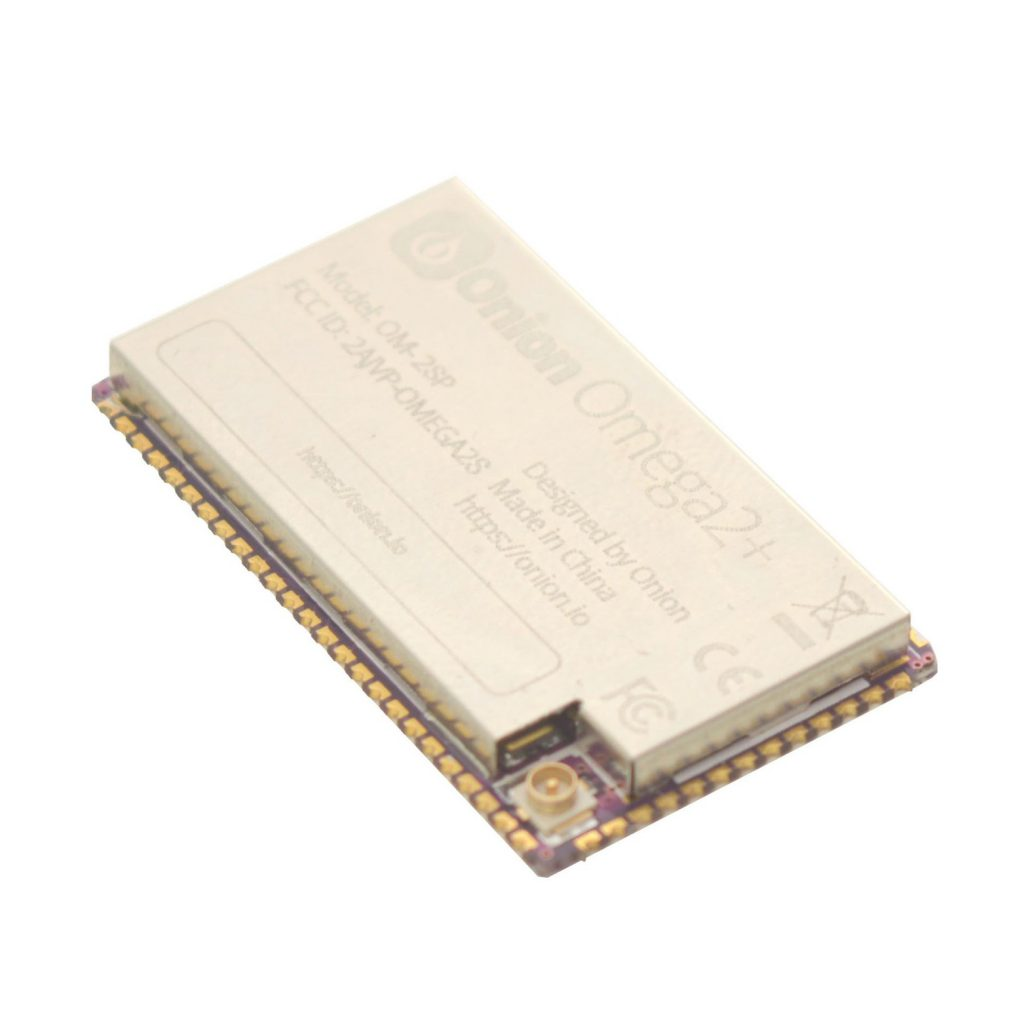
\includegraphics[width=.3\textwidth]{img/Omega2S.jpg}}
    \subfloat[\label{fig:RN4871} RN4871 \cite{microchip_technology_inc_rn4871_nodate}]{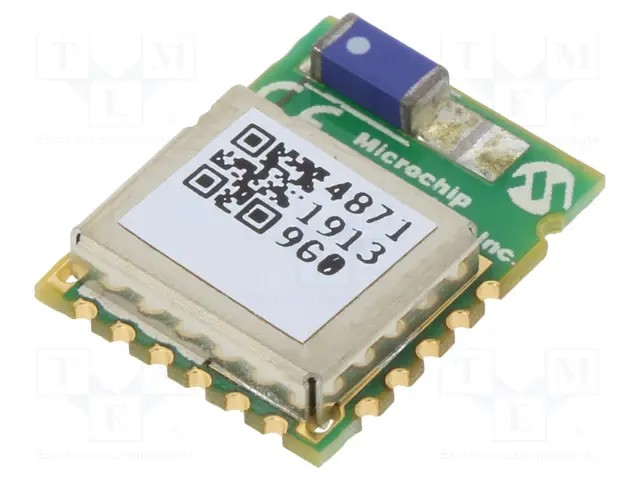
\includegraphics[width=.3\textwidth]{img/rn4871.jpg}}
    \subfloat[MAX F10s \cite{u-blox_max-f10s_2024}]{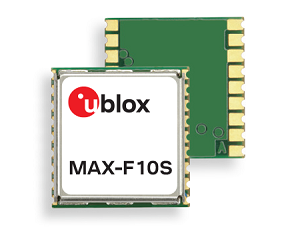
\includegraphics[width=.3\textwidth]{img/max-f10s.png}}
    \caption{\label{fig:wireless-modules} Examples of common wireless modules}
\end{figure}

This approach allows us to separate the usually complex and more expensive multi-layer board layouts, required by modern SOCs, along with their power delivery and any other supporting circuitry, from the less complex end-application consisting of local power regulation, battery management, connectors and other mechanical features.

In order to satisfy the requirements \ref{section:final-requirements}, the module should provide means for analog and digital signal acquisition, digital communication interfaces and sufficient internal storage along with implementing the wireless connectivity.

\subsection{\label{section:mcu}Microcontroller}
Given the requirements for minimal footprint a fully integrated SOC solution is preferred to a configuration of separate MCU and an RF solution. STM32WL series offers such an SOC, which also satisfies the requirement of low power consumption by being based on the STM32L4, a well known ultra low power family of micro-controllers.

The manufacturer also offers a development board, the NUCLEO-WL55JC (\ref{fig:nucleo}), and a plethora of reference designs, the STDES-WL5xxxxx series, where the STDES-WL5U4ILH (\ref{fig:reference-design}) overlaps well with our requirements.

\begin{figure}
    \centering
    \subfloat[\label{fig:nucleo} NUCLEO-WL55JC \cite{stmicroelectronics_nucleo-wl55jc_2024}]{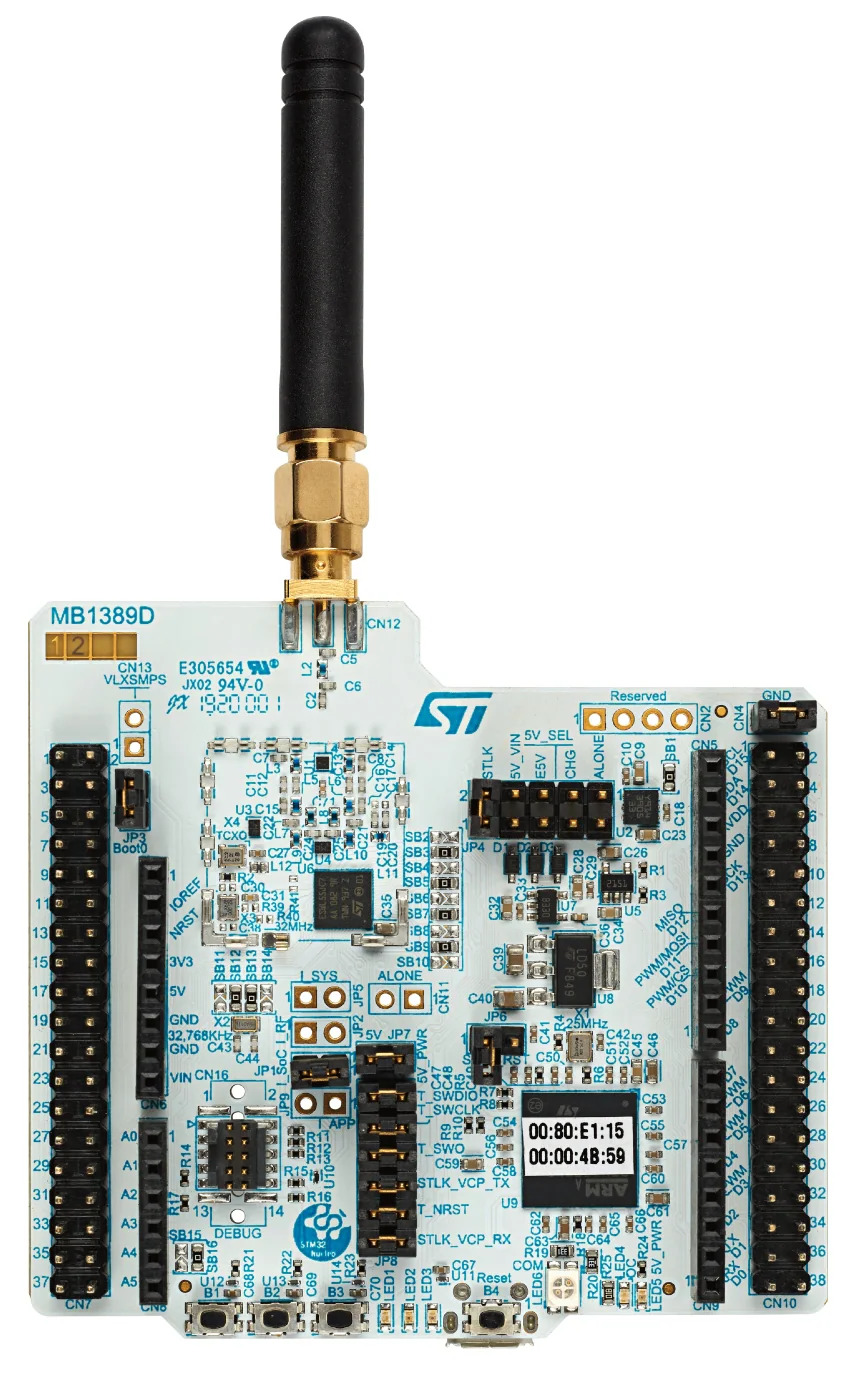
\includegraphics[width=.3\textwidth]{img/nucleo-wl55jc.jpg}}
    \subfloat[\label{fig:reference-design} STDES-WL5U4ILH \cite{stmicroelectronics_stdes-wl5u4ilh_2024}]{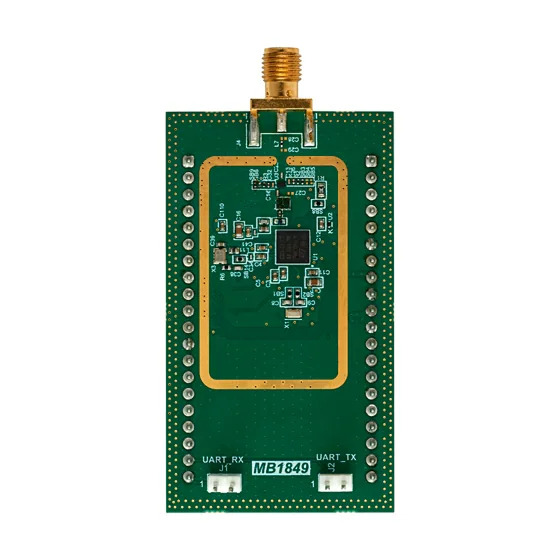
\includegraphics[width=.5\textwidth]{img/STDES-WL5U4ILH.jpg}}
    \caption{\label{fig:nucleo-and-reference} Nucleo development kit and the reference design board}
\end{figure}

Each of the designs focuses on optimizing different parameters depending on the application priorities and their codification follows table \ref{fig:reference-design-codification}, from which the defining features are apparent. For this work, application footprint was one of the top priorities, so the lower-power $15~\mathrm{dB}$ version with IPD was selected.

IPD stands for Integrated Passive Device, it consists of a balun and a harmonic filter. This circuitry is usually realized using passive components, which is cheaper, but takes up more board space (see Figure \ref{fig:frontend-comparison} for comparison), is more prone to design mistakes and tuning mismatch. This particular IPD was specifically designed for STM32WL line of microcontrollers in this configuration \cite{stmicroelectronics_balfhb-wl-05d3_2024}.

\begin{figure}
    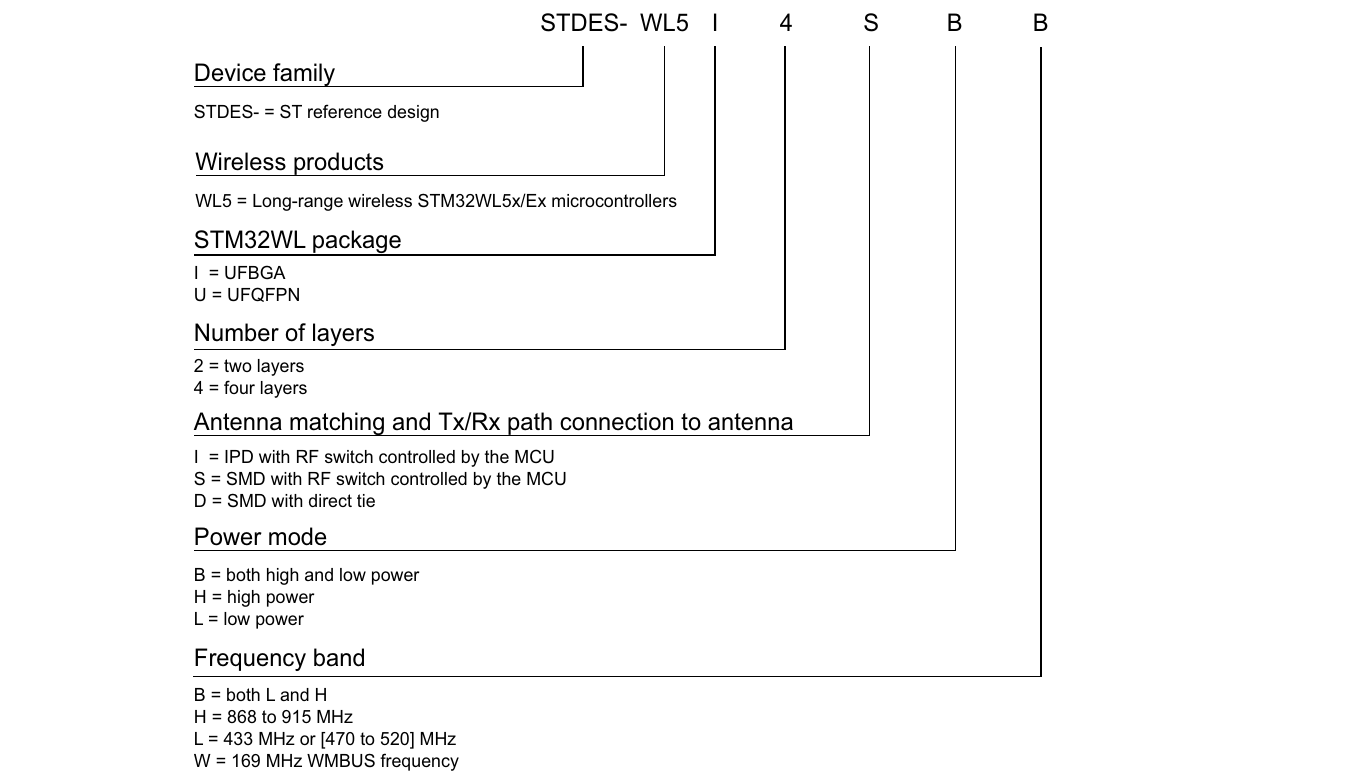
\includegraphics[width=\textwidth]{fig/STDES-xxxxxxx.png}
    \caption{\label{fig:reference-design-codification} STM32WL5x and STM32WLEx reference designs codification}
\end{figure}

\begin{figure}
    \centering
    \subfloat[discrete /wo RF switch (variant D)]{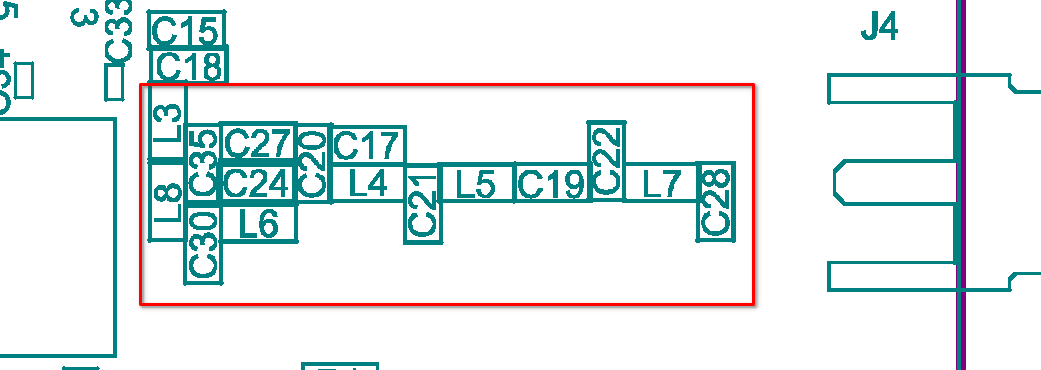
\includegraphics[angle=-90,width=.21\textwidth]{img/frontend-dlb.png}}\hfil
    \subfloat[discrete /w RF switch (variant S)]{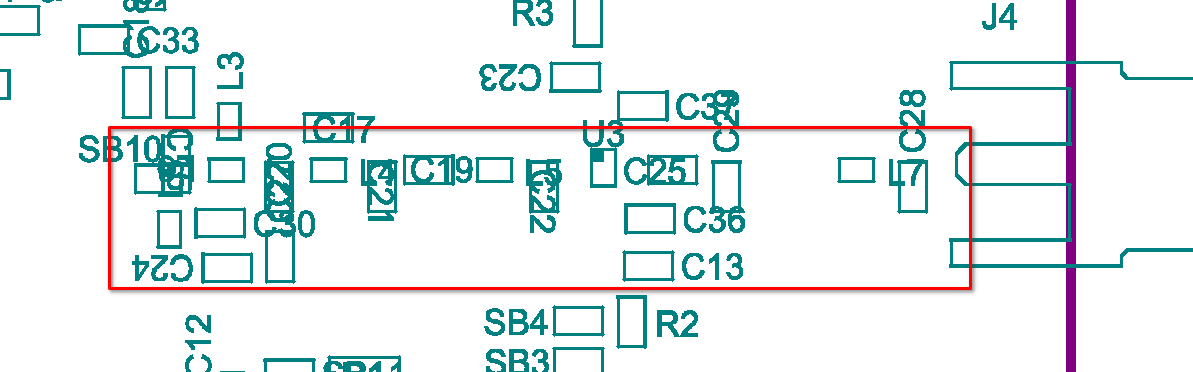
\includegraphics[angle=-90,width=.19\textwidth]{img/frontend-sbb.png}}\hfil
    \subfloat[IPD (variant I)]{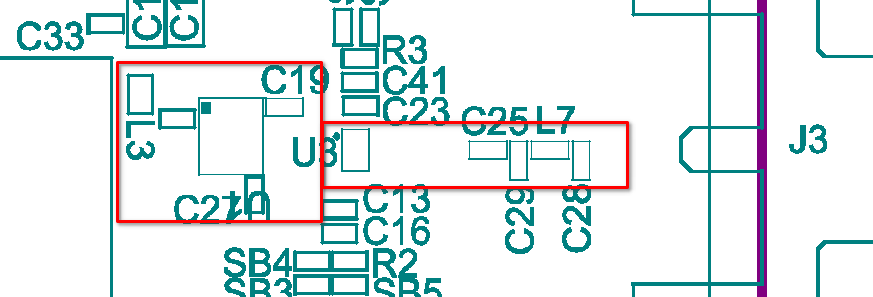
\includegraphics[angle=-90,width=.21\textwidth]{img/frontend-ilh.png}}
    \caption{\label{fig:frontend-comparison} Frontend layout and part selection comparison, components on the RF path highlighted. Reference designs selected for comparison were picked based on the similarity with the STDES-WL5U4ILH design.}
\end{figure}

One downside of using an IPD in this case is that it requires the use of an RF switch, because ST's IPDs are designed to work with separate receive and transmit paths. Again this is a tradeoff between complexity, cost and board space required. Fortunately only a Single Pole Double Throw switch is required, thus a simple switch such as the BGS12SN6 from Infineon \cite{infineon_technologies_bgs12sn6_2024} is sufficient.

A 4 layer reference design was selected because it is anticipated it will allow a higher density layout, shrinking the module dimensions even further. UFQFPN package is preferred over UFBGA to stay compatible with lower cost manufacturing solutions. It is expected the design will use most of the available pins on the package, a complex fanout would be required if we were to go with the BGA variant, perhaps some space savings could be had at the cost of losing access to most of the pins, making any modifications to the design difficult to impossible, should the need arise.

In conclusion, the MCU choice is a culmination of tradeoffs, where the prevention of mistakes, efficiency and familiarity were more important than the absolute performance and cost. This should not in any way hamper further improvements in succeeding versions of this hardware, while allowing the completion of Proof-of-Concept stages of this project. 

\subsection{Power regulation and standby mode solution}
The selected MCU supports wide input voltage of $2\text{--}3.6~\mathrm{V}$ thanks to its internal voltage regulation. It supports two modes - LDO, which does not require any additional external component at the cost of lower efficiency and the SMPS mode, utilizing a synchronous buck regulator, which is more efficient - this application will therefor attempt to implement the latter.

A separate, switchable power-rail is a feature deemed necessary by some considered applications in \ref{section:application-case-studies}. This can be achieved using a built-in MOSFET - such power rail could be used to save power even by powering off some parts of the module itself.

\subsection{Integrated non-volatile memory}
As outlined in the OTA update support section \ref{section:ota-update-support}, an external memory is needed to store the application binary during the download process. This memory does not need to be non-volatile, but since it is comparatively cheaper than RAM and provides a backup in case of a power loss, the choice is apparent.

LoRa data rates are in the realm of 100--1000 bytes per second, even less in real-world applications, thus basically any available interface can be used. The capacity needs to be at-least equal to the built-in FLASH memory of the MCU \ref{section:mcu}, which is $256~\mathrm{kB}$.

The SST26VF080A $8~\mathrm{Mb}$ FLASH memory was selected. It is available in the WDFN-8 package, which is space-efficient, features a standard SPI interface and supports a wide input voltage range of $2.3\text{--}3.6~\mathrm{V}$, which was an important consideration for this use-case.

\subsection{\label{section:antenna}Antenna}
In the initial module requirements \ref{section:final-requirements} it was deemed preferable to integrate the antenna onto the module itself. This should not, however, compromise on the usability and performance of the module. 

In general, there are two approaches for integrated antennae - a trace antenna constructed using the PCB directly, or an antenna in the form of a solderable component, such as an ceramic chip antenna. If the board space is limited, the performance is insufficient or the use of an integrated antenna is prohibited by any other limitation, the application must resort to an external antenna connected to the RF circuitry through a coaxial cable. The table \ref{table:antenna-solutions} provides a summary.

\begin{table}[H]
\begin{center}
\caption{\label{table:antenna-solutions}Summary of advantages and disadvantages of different antenna solutions according to \cite{andersen_selecting_2008}}
    \begin{tabular}{|l|l|l|}
    \hline
    \textbf{Antenna types} & \textbf{Advantages} & \textbf{Disadvantages} \\
    \hline
    PCB antenna  & Low cost, No assembly,        & Difficult to design small \\
                 & Good performance achievable,  & and efficient antenna, \\
                 & Small size at high frequency  & Large size at low frequency \\
    \hline
    Chip antenna & Small size,                   & Medium performance, \\
                 & Off-the-shelf solution        & Medium cost \\
    \hline
    Whip (external)& Good performance,           & High cost, \\
    antenna        & Off-the-shelf solution      & Large size \\
    \hline
    \end{tabular}
\end{center}
\end{table}

The following sections elaborate on each antenna type in more detail in the context of this particular application. 

At this point in the design process, the module proportions, derived from the individual component footprints, are not expected to surpass $500~\mathrm{mm^2}$. It is also expected the design will need to conform to the PCB parameters specified in Table \ref{table:pcb-parameters}. Since the first prototypes will only operate in Europe, the aim is mainly the EU868 band.

\begin{table}[H]
\begin{center}
\caption{\label{table:pcb-parameters}PCBWay manufacturer stackup parameters \cite{pcbway_stackup_2024}}
    \begin{tabular}{|l|l|} \hline
    \textbf{Parameter}            & \textbf{Value} \\ \hline
    Stackup thickness             & $1.6~\mathrm{mm}$ \\ \hline
    Substrate dielectric constant & $4.5~\mathrm{[-]}$ \\ \hline
    Substrate loss tangent        & $0.02~\mathrm{[-]}$ \\ \hline
    \end{tabular}
\end{center}
\end{table}

\subsubsection{Printed Circuit Board antenna}
Due to the limited board space, this option is expected to not be feasible. Nevertheless, some types of PCB antenna solutions were calculated to support this intuition.

A microstrip patch antenna is one of the simplest types of PCB antenna designs \cite{zachariah_peterson_microstrip_2022,wallace_an058_nodate}. This antenna consists of the patch itself and its feed-line with optional inset for impedance matching, see \ref{fig:patch-antenna}. 

The approximate parameters presented in Table \ref{table:antenna-pcb-calculations} were obtained using \cite{zachariah_peterson_microstrip_2022}, the input impedance could be tuned using the inset and a matching circuit, but more importantly, this simple antenna design is not practical because of its size, which already has roughly 15 times the surface area of the module components.

Another, more space-efficient option, is to use the inverted-F design, see Figure \ref{fig:inverted-f-antenna} for its simplest form. We can calculate its length $L$ given the target frequency $f$
\begin{equation}
    % 299,792,458/(4*868,000,000)
    L = \dfrac{\lambda}{4} = \dfrac{c_0}{4f} = \dfrac{c_0}{4 \cdot 868 \cdot 10^6} \approx 86.3~\mathrm{mm}
\end{equation}
which is a great improvement compared to the patch antenna.

This design could perhaps be optimized such that it would fit the size constraints, but such work might be enough to write another thesis focused on just this detail. Dimensions based on the layout in Figure \ref{fig:inverted-f-antenna} were included in Table \ref{table:antenna-pcb-calculations} for comparison sake.

\begin{figure}
    \centering
    \subfloat[\label{fig:patch-antenna}Microstrip patch antenna dimensions including the feed-line \cite{zachariah_peterson_microstrip_2022}]{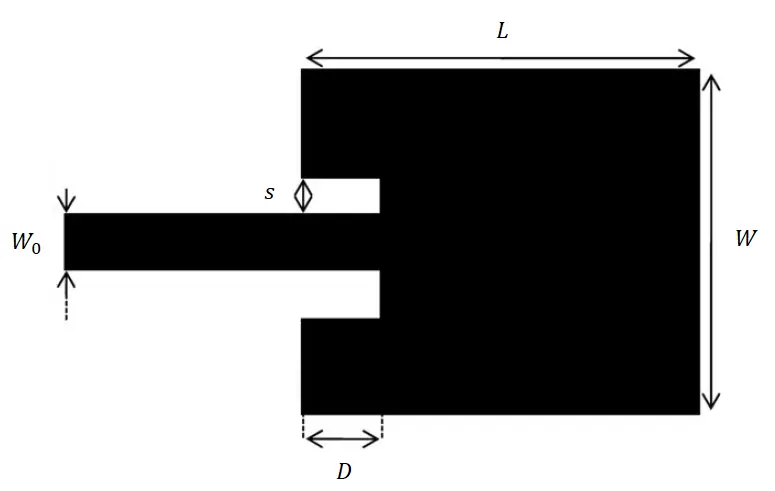
\includegraphics[width=.53\textwidth]{fig/patch-antenna.png}}\hfill
    \subfloat[\label{fig:inverted-f-antenna}Basic inverted-F antenna design \cite{peterson_inverted-f_2023}]{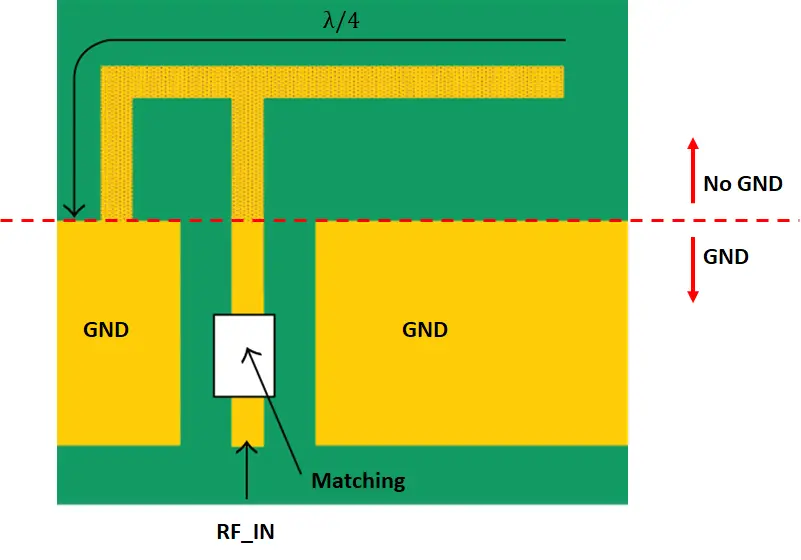
\includegraphics[width=.43\textwidth]{fig/inverted-f-antenna.png}}
    \caption{Simple Printed Circuit Board antenna designs}
\end{figure}

\begin{table}[H]
\begin{center}
\caption{\label{table:antenna-pcb-calculations}Approximate microstrip patch antenna parameters and dimensions (as described in \ref{fig:patch-antenna}) and a notion of the dimensions of an inverted-F antenna (corresponding to \ref{fig:inverted-f-antenna}), not including the ground-plane and matching network}
    \begin{tabular}{|l|l|l|} \hline
    \textbf{Parameter}  & \textbf{Patch antenna}    & \textbf{Inverted-F antenna} \\ \hline
    Input impedance     & $306~\mathrm{\Omega}$     & not calculated \\ \hline
    Bandwidth           & $3.92~\mathrm{MHz}$       & not calculated \\ \hline
    Width (W)           & $104~\mathrm{mm}$         & $\approx 70~\mathrm{mm}$ \\ \hline
    Length (L)          & $80~\mathrm{mm}$          & $\approx 18~\mathrm{mm}$ \\ \hline
    Minimum footprint   & $8320~\mathrm{mm^2}$      & $1260~\mathrm{mm^2}$ \\ \hline
    \end{tabular}
\end{center}
\end{table}

These preliminary calculations led to the conclusion, that a PCB antenna at this frequency with these size constraints is not viable in this case. These calculations are not even beginning to factor in all the other components required, not to mention the even larger ground-plane which such antenna would require. 

This could be made possible with significant design effort and expertise, or by licensing an existing design, but the overall goal of creating this hardware would need to shift as a result.

\subsubsection{Chip antenna}
As outlined in \ref{table:antenna-solutions}, the chip antenna is another logical step in the search of the right solution. It is a common choice seen in commercially available hardware, especially in cases, where the space is at a premium - as can be seen on the RN4871 \ref{fig:RN4871} Bluetooth module.

There is a large selection of these antennae on the market, mainly targeted at the very common bands, such as $2.4~\mathrm{GHz}$ and $5~\mathrm{GHz}$, but solutions for the $868~\mathrm{MHz}$ frequency range are also not hard to come by \cite{digikey_rf_2024,mouser_europe_868_2024}.

The search was narrowed by focusing on omnidirectional and linearly polarized antennae of small size and straightforward implementation guidelines. Cost also played a factor, since many solutions, although good, would make the design unfeasible.

The following Table \ref{table:antenna-chip} features the main candidates that were picked. All have $50~\mathrm{\Omega}$ impedance and satisfy the above criteria.

\begin{table}[H]
\begin{center}
\caption{\label{table:antenna-chip}Comparison of the three selected chip antennae}
    \begin{tabular}{|l|l|l|l|} \hline
    \textbf{Parameter} & \textbf{Linx ANT868}\cite{linx_technologies_he_2024} & \textbf{Kyocera M6207}\cite{kyocera_ism_2024} & \textbf{Taoglas ILA08}\cite{taoglas_ila08_nodate} \\ \hline
    Construction & Wire wound & Ceramic chip & Ceramic chip \\ \hline
    Rated frequency                 & $862 \text{--} 876~\mathrm{MHz}$ & $863 \text{--} 870~\mathrm{MHz}$ & $863 \text{--} 870~\mathrm{MHz}$ \\ \hline
    Peak gain                       & $5.6~\mathrm{dB}$     & $0.3~\mathrm{dB}$     & $-0.5~\mathrm{dB}$ \\ \hline
    Average gathering               & $-1.1~\mathrm{dB}$    & $-5.0~\mathrm{dB}$    & $-4.0~\mathrm{dB}$ \\ \hline
    Maximum VSWR                    & $2.2$                 & $1.7$                 & $1.9$ \\ \hline
    Dimensions $\mathrm{[mm]}$      & $25.4 \times 15.3 \times 8.9$ & $6.0 \times 2.0 \times 1.0$ & $5.0 \times 3.0 \times 0.5$ \\ \hline
    Ground plane $\mathrm{[mm]}$    & $84.0 \times 38.0$ & $100.0 \times 40.0$ & $80.0 \times 40.0$ \\ \hline
    \end{tabular}
\end{center}
\end{table}

\subsubsection{External antenna}
It was deemed necessary to rely on an external antenna instead of an integrated on-module antenna. This choice was done primarily because of the ground plane requirements of the integrated solutions, which is a downside of using lower frequencies in general.

Size of the ground-plane has a large affect on the antenna performance and its tuning. Due to the nature of a communications module, which could be used in different applications, these requirements would need to be closely followed by the application, failing that could cause the module to radiate outside of the intended frequency range.

External antenna has the major advantage of being self-contained, thus the implications on the circuit board design are minimal and the responsibility is shifted onto the placement of the antenna, providing enough clearance and using RF-transparent materials.

Another advantage, for the use in soil moisture sensing, is that the antenna can be mounted higher above the ground level, which could improve its performance significantly if long-range transmission is required.

\subsection{Conclusion}
During the component selection phase, the requirements set in \ref{section:final-requirements} were continually assessed and successfully met. One major compromise was made in the antenna selection, where the design needed to resort to an externally connected antenna due to the size and application constraints. This choice however should ensure that the potential for problems arising during prototype stages should be limited.

\FloatBarrier
\section{Sensor architecture}
Given that the primary point of this work is to create a proof-of-concept sensing solution, which utilizes the LoRa module envisioned in \ref{section:module-architecture}, the sensor should be suitable for small-scale testing and prototype work, it should also be simple to manufacture and maximize the potential for success in the first iteration, due to the limited time allocated for the whole project.

A single board construction is suitable, as it is simple, self-contained and can be made through standard PCB manufacturers. It is also commonly seen in hobby grade and some commercial soil moisture sensors.

\subsection{Expected capacitance range}

\subsection{Measuring method}

\subsection{Battery and charging}
